\documentclass{Configuration_Files/PoliMi3i_thesis}

% CONFIGURATIONS
\usepackage{parskip} % For paragraph layout
\usepackage{setspace} % For using single or double spacing
\usepackage{emptypage} % To insert empty pages
\usepackage{multicol} % To write in multiple columns (executive summary)
\setlength\columnsep{15pt} % Column separation in executive summary
\setlength\parindent{0pt} % Indentation
\raggedbottom  

% PACKAGES FOR TITLES
\usepackage{titlesec}
% \titlespacing{\section}{left spacing}{before spacing}{after spacing}
\titlespacing{\section}{0pt}{3.3ex}{2ex}
\titlespacing{\subsection}{0pt}{3.3ex}{1.65ex}
\titlespacing{\subsubsection}{0pt}{3.3ex}{1ex}
\usepackage{color}

% PACKAGES FOR LANGUAGE AND FONT
\usepackage[english]{babel} % The document is in English  
\usepackage[utf8]{inputenc} % UTF8 encoding
\usepackage[T1]{fontenc} % Font encoding
\usepackage[11pt]{moresize} % Big fonts

% PACKAGES FOR IMAGES 
\usepackage{graphicx}
\usepackage{transparent} % Enables transparent images
\usepackage{eso-pic} % For the background picture on the title page
\usepackage{subfig} % Numbered and caption subfigures using \subfloat.
\usepackage{tikz} % A package for high-quality hand-made figures.
\usetikzlibrary{}
\graphicspath{{./Images/}} % Directory of the images
\usepackage{caption} % Coloured captions
\usepackage{xcolor} % Coloured captions
\usepackage{amsthm,thmtools,xcolor} % Coloured "Theorem"
\usepackage{float}

% STANDARD MATH PACKAGES
\usepackage{amsmath}
\usepackage{amsthm}
\usepackage{amssymb}
\usepackage{amsfonts}
\usepackage{bm}
\usepackage[overload]{empheq} % For braced-style systems of equations.
\usepackage{fix-cm} % To override original LaTeX restrictions on sizes

% PACKAGES FOR TABLES
\usepackage{tabularx}
\usepackage{longtable} % Tables that can span several pages
\usepackage{colortbl}

% PACKAGES FOR ALGORITHMS (PSEUDO-CODE)
\usepackage{algorithm}
\usepackage{algorithmic}

% PACKAGES FOR REFERENCES & BIBLIOGRAPHY
\usepackage[
	colorlinks=true,
	linkcolor=black,
	anchorcolor=black,
	citecolor=black,
	filecolor=black,
	menucolor=black,
	runcolor=black,
	urlcolor=black
]{hyperref} % Adds clickable links at references
\usepackage{cleveref}
\usepackage[square, numbers, sort&compress]{natbib} % Square brackets, citing references with numbers, citations sorted by appearance in the text and compressed
\bibliographystyle{abbrvnat} % You may use a different style adapted to your field

% OTHER PACKAGES
\usepackage{pdfpages} % To include a pdf file
\usepackage{afterpage}
\usepackage{lipsum} % Dummy package
\usepackage{fancyhdr} % For the headers
\usepackage{enumitem}
\fancyhf{}
\usepackage{listingsutf8}
\usepackage{xcolor}

% Input of configuration file. Do not change config.tex file unless you really know what you are doing. 
% Define blue color typical of polimi
\definecolor{bluepoli}{cmyk}{0.4,0.1,0,0.4}

% Custom theorem environments
\declaretheoremstyle[
  headfont=\color{bluepoli}\normalfont\bfseries,
  bodyfont=\color{black}\normalfont\itshape,
]{colored}

% Set-up caption colors
\captionsetup[figure]{labelfont={color=bluepoli}} % Set colour of the captions
\captionsetup[table]{labelfont={color=bluepoli}} % Set colour of the captions
\captionsetup[algorithm]{labelfont={color=bluepoli}} % Set colour of the captions

\theoremstyle{colored}
\newtheorem{theorem}{Theorem}[chapter]
\newtheorem{proposition}{Proposition}[chapter]

% Enhances the features of the standard "table" and "tabular" environments.
\newcommand\T{\rule{0pt}{2.6ex}}
\newcommand\B{\rule[-1.2ex]{0pt}{0pt}}

% Pseudo-code algorithm descriptions.
\newcounter{algsubstate}
\renewcommand{\thealgsubstate}{\alph{algsubstate}}
\newenvironment{algsubstates}
  {\setcounter{algsubstate}{0}%
   \renewcommand{\STATE}{%
     \stepcounter{algsubstate}%
     \Statex {\small\thealgsubstate:}\space}}
  {}

% New font size
\newcommand\numfontsize{\@setfontsize\Huge{200}{60}}

% Title format: chapter
\titleformat{\chapter}[hang]{
\fontsize{50}{20}\selectfont\bfseries\filright}{\textcolor{bluepoli} \thechapter\hsp\hspace{2mm}\textcolor{bluepoli}{|   }\hsp}{0pt}{\huge\bfseries \textcolor{bluepoli}
}

% Title format: section
\titleformat{\section}
{\color{bluepoli}\normalfont\Large\bfseries}
{\color{bluepoli}\thesection.}{1em}{}

% Title format: subsection
\titleformat{\subsection}
{\color{bluepoli}\normalfont\large\bfseries}
{\color{bluepoli}\thesubsection.}{1em}{}

% Title format: subsubsection
\titleformat{\subsubsection}
{\color{bluepoli}\normalfont\large\bfseries}
{\color{bluepoli}\thesubsubsection.}{1em}{}

% Shortening for setting no horizontal-spacing
\newcommand{\hsp}{\hspace{0pt}}

\makeatletter
% Renewcommand: cleardoublepage including the background pic
\let\cleardoublepage\clearpage

%For correctly numbering algorithms
\numberwithin{algorithm}{chapter}

%----------------------------------------------------------------------------
%	BEGIN OF YOUR DOCUMENT
%----------------------------------------------------------------------------

\begin{document}

\fancypagestyle{plain}{%
\fancyhf{} % Clear all header and footer fields
\fancyhead[RO,RE]{\thepage} %RO=right odd, RE=right even
\renewcommand{\headrulewidth}{0pt}
\renewcommand{\footrulewidth}{0pt}}

%----------------------------------------------------------------------------
%	TITLE PAGE
%----------------------------------------------------------------------------

\pagestyle{empty} % No page numbers
\frontmatter % Use roman page numbering style (i, ii, iii, iv...) for the preamble pages

\puttitle{
	title={IoT Challenge \#2,\\Exercise Application Layer},% Title of the thesis
	course={Internet of Things},
	name1={Kevin Ziroldi - 10764177},
	name2={Matteo Volpari - 10773593},
	advisors= {Alessandro Redondi, Fabio Palmese}, % Supervisor name
	academicyear={2024-2025},  % Academic Year
	version={1.0}, 
	releasedate={6-4-2025}
} 
          
%----------------------------------------------------------------------------
%	PREAMBLE PAGES: ABSTRACT (inglese e italiano), EXECUTIVE SUMMARY
%----------------------------------------------------------------------------
\startpreamble
\setcounter{page}{1} % Set page counter to 1

%----------------------------------------------------------------------------
%	LIST OF CONTENTS/FIGURES/TABLES/SYMBOLS
%----------------------------------------------------------------------------

% TABLE OF CONTENTS
\thispagestyle{empty}
\tableofcontents % Table of contents 
\thispagestyle{empty}
\cleardoublepage

%-------------------------------------------------------------------------
%	THESIS MAIN TEXT
%-------------------------------------------------------------------------
% In the main text of your thesis you can write the chapters in two different ways:
%
%(1) As presented in this template you can write:
%    \chapter{Title of the chapter}
%    *body of the chapter*
%
%(2) You can write your chapter in a separated .tex file and then include it in the main file with the following command:
%    \chapter{Title of the chapter}
%    \input{chapter_file.tex}
%
% Especially for long thesis, we recommend you the second option.

% The \label{...}% enables to remove the small indentation that is generated, always leave the % symbol.

\addtocontents{toc}{\vspace{2em}} % Add a gap in the Contents, for aesthetics
\mainmatter % Begin numeric (1,2,3...) page numbering

% --------------------------------------------------------------------------
% NUMBERED CHAPTERS % Regular chapters following
% --------------------------------------------------------------------------

\chapter{Exercise temperature sensor and valve}
\label{ch:chapter_one}%
\subsubsection{Data}

The data of the exercise is reported here.
\begin{itemize}
	\item 10 sensors
	\item $T_{transmission} = 10 \text{ minutes}$
	\item $b = 2000 \text{ bit}$
	\item $E_b = 5 \text{ mJ}$
	\item $E_c = 50 \text{ nJ/bit}$
	\item $E_{tx}(d) = k \cdot d^2 \text{ nJ/bit}$
	\item $k = 1 \text{ nJ/bit/$m^2$}$
\end{itemize}

The sensors of the parking lot have fixed positions, reported in the following table.
\begin{table}[H]
\centering 
\begin{tabular}{| c | c |}
	\hline 
	\rowcolor{bluepoli!40}
	\textbf{Sensor} & \textbf{Position}\T\B \\
	\hline 
	1 & (1, 2) \T\B\\
	2 &(10, 3) \T\B\\
	3 & (4, 8) \T\B\\
	4 & (15, 7) \T\B\\
	5  & (6, 1) \T\B\\
	6  & (9, 12) \T\B\\
	7  & (14, 4) \T\B\\
	8  & (3, 10) \T\B\\
	9  & (7, 7) \T\B\\
	10  & (12, 14) \T\B\\
	\hline
\end{tabular}
\\[10pt]
\caption{Sensor position table}
\label{table:sensor_position_table}
\end{table}

The following picture describes the distributions of sensors.
\begin{figure}[H]
    \centering
    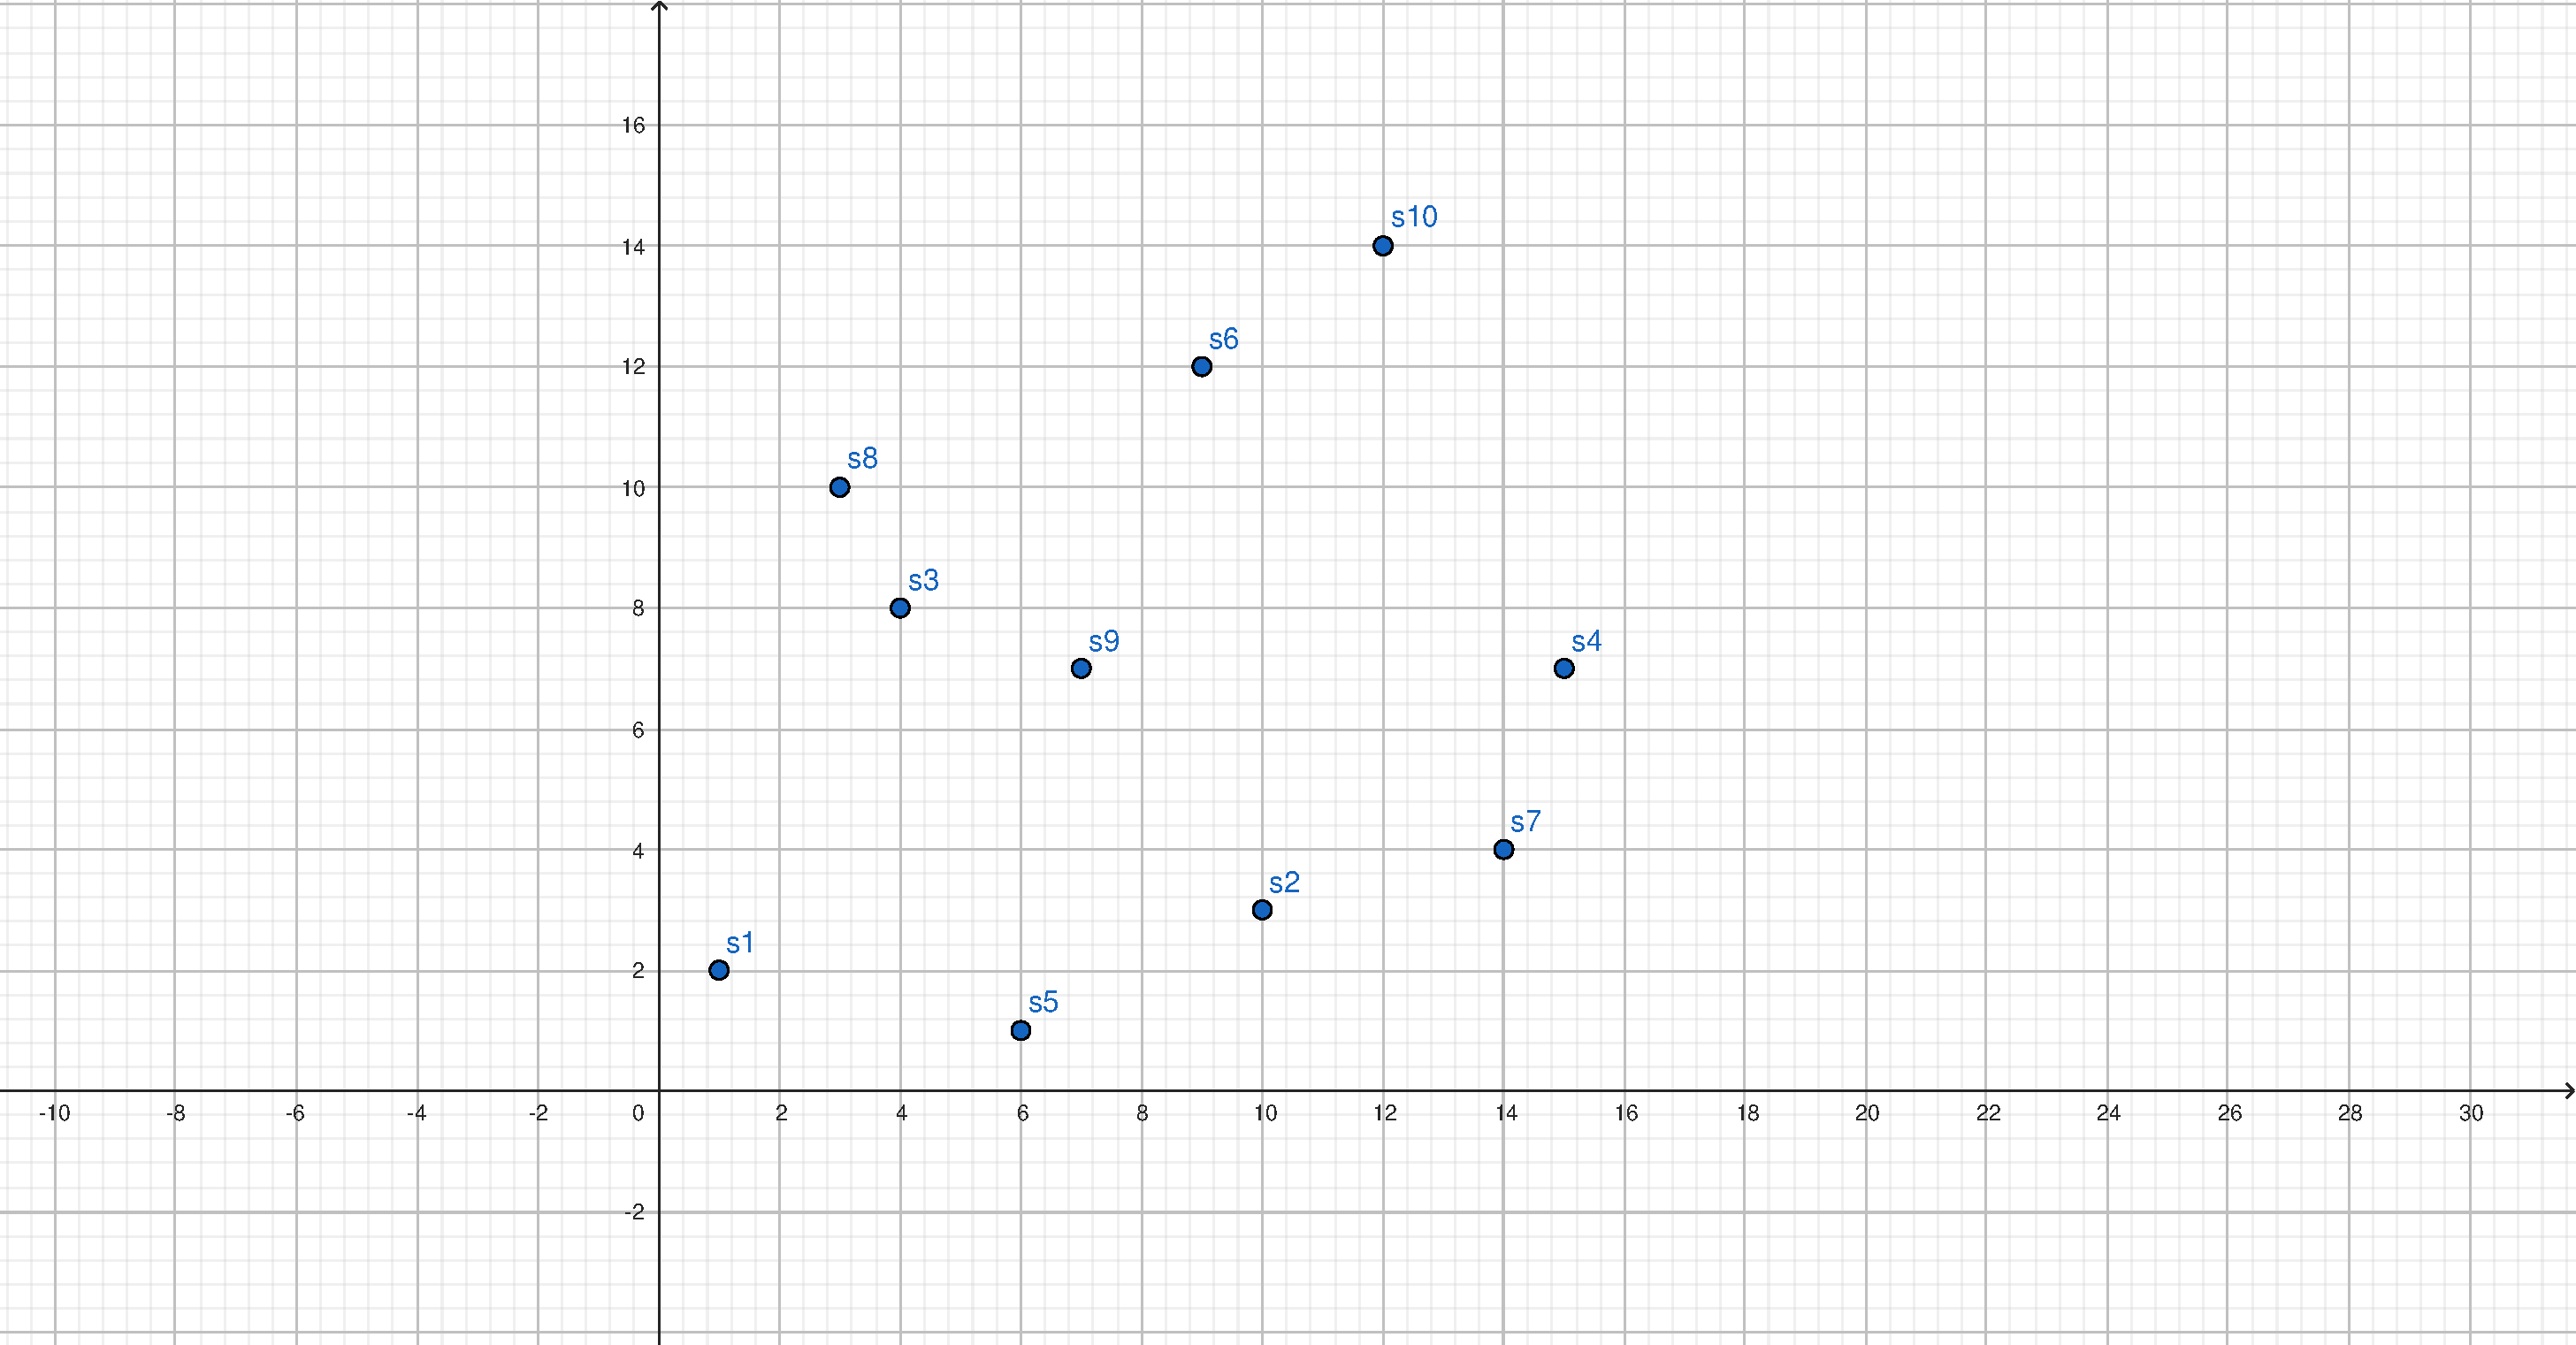
\includegraphics[width=\linewidth, height=0.3\textheight, keepaspectratio]{points.pdf}
    \caption{Sensor distribution}
    \label{fig:Sensor_distribution}
\end{figure}


\subsubsection{Lifetime of the system with sink in (20,20)}
In order to compute the lifetime of the system when the sink position is ($x_s, y_s$) = (20, 20), we need to compute the lifetime of the furthest sensor from the sink.\\
We calculated the distance of every sensor from the sink, the values are reported in the following table.

\begin{table}[H]
\centering 
\begin{tabular}{| c | c | c |}
	\hline 
	\rowcolor{bluepoli!40}
	\textbf{Sensor} & \textbf{Position} & \textbf{Distance from sink}\T\B \\
	\hline 
	1 & (1, 2) & $\sqrt{685} \text{ m}$ \T\B\\
	2 &(10, 3) & $\sqrt{389} \text{ m}$ \T\B\\
	3 & (4, 8) & 20 m\T\B\\
	4 & (15, 7) & $\sqrt{194} \text{ m}$ \T\B\\
	5  & (6, 1) & $\sqrt{557} \text{ m}$ \T\B\\
	6  & (9, 12) & $\sqrt{185} \text{ m}$ \T\B\\
	7  & (14, 4) & $2\sqrt{73} \text{ m}$ \T\B\\
	8  & (3, 10) & $\sqrt{389} \text{ m}$ \T\B\\
	9  & (7, 7) & $13\sqrt{2} \text{ m}$ \T\B\\
	10  & (12, 14) & 10 m\T\B\\
	\hline
\end{tabular}
\\[10pt]
\caption{Distances from sink}
\end{table}

The distance between the sink and the furthest sensor, sensor 1, is: 
\[ 
distance_1 = d \{(1, 2) , (20, 20)\} = \sqrt{(20-1)^2 + (20-2)^2} = \sqrt{685} m 
\]
We compute the energy consumed by sensor 1 as:
\[
E_{cycle, 1} = E_c \cdot b + E_{tx, 1}(d) \cdot b = 50 nJ/bit \cdot 2000 \text{ bit} + 1 nJ/bit/m^2 \cdot 685 m^2 \cdot 2000 \text{ bit} = 1.47 mJ
\]
The lifetime, measured in number of cycles, is:
\[
L_{cycles} = E_b / E_{cycle, 1} = 3.401 \text{ cycles}
\]
Assuming that each sensor transmits at the beginning of the ten minutes, the system will last for three cycles and during the fourth cycle the furthest sensor will die.

\subsubsection{Optimal sink position}
In order to maximize the system's lifetime, we need to maximize the lifetime of the sensor node that consumes the most energy. The energy consumption for a transmission is given by:
\[
E_{cycle} = E_c \cdot b + E_{tx}(d) \cdot b = E_c \cdot b + k \cdot d^2 \cdot b
\]
Since the energy for the circuitry, $E_c$, is constant, the energy consumption grows with the distance. In order to maximize the lifetime of the system, we need to minimize the maximum distance between the sink and the furthest node. This problem is equivalent to that of finding the smallest circle enclosing all point on the cartesian plane, representing the positions of nodes.\\
A very efficient algorithm that can be used to solve the smallest enclosing circle problem is Welzl's algorithm, which finds a solution in O(n) time. 
The algorithm is recursive and uses two sets:
\begin{itemize}
	\item P: contains all input points;
	\item R: initially empty, at the end, contains point on the boundary of the minimum enclosing circle;
\end{itemize}
The base cases are the ones in which the smallest circle encloses three or less points:
\begin{itemize}
	\item if it doesn't enclose any point, the circle is undefined;
	\item if it encloses one point, the degenerate circle is the point itself and has radius zero;
	\item if it encloses two points or three points, there is just one circle passing through them;
\end{itemize}
At each step, select a point p from P and find the smallest enclosing circle of the other points:
\begin{itemize}
	\item  if p lies in D, D is the minimum enclosing circle;
	\item otherwise, p must be part of the boundary, remove p from P and add it to R, recurse on the next element of set P;
\end{itemize}
A Python implementation of the algorithm can be found below.

\begin{python}
import math
import random

# data structures
class Point:
    def __init__(self, x, y):
        self.x = x
        self.y = y

class Circle:
    def __init__(self, c, r):
        self.c = c
        self.r = r

# checks wheter point p is inside circle c 
def isInside(c, p):
    return math.dist([c.c.x, c.c.y], [p.x, p.y]) <= c.r

# checks if all points in ps are in c 
def isValidCircle(c, ps):
    return all(isInside(c, point) for point in ps)

# helper method to get a circle defined by 3 points
def getCircleCenter(bx, by, cx, cy):
    b = bx * bx + by * by
    c = cx * cx + cy * cy
    d = bx * cy - by * cx
    return Point((cy * b - by * c) / (2 * d), (bx * c - cx * b) / (2 * d))

# returns the circle passing for 2 points (a,b)
def circleFromTwo(a, b):
    c = Point((a.x + b.x) / 2.0, (a.y + b.y) / 2.0)
    return Circle(c, math.dist([a.x, a.y], [b.x, b.y]) / 2.0)

# returns the circle passing for 3 points (a,b,c)
def circleFromThree(a, b, c):
    i = getCircleCenter(b.x - a.x, b.y - a.y, c.x - a.x, c.y - a.y)
    i.x += a.x
    i.y += a.y
    return Circle(i, math.dist([i.x, i.y], [a.x, a.y]))

# minimum enclosing circle trivial cases
def minCircleTrivial(p):
    assert len(p) <= 3
    if not p:
        return Circle(Point(0, 0), 0)
    elif len(p) == 1:
        return Circle(p[0], 0)
    elif len(p) == 2:
        return circleFromTwo(p[0], p[1])

    for i in range(3):
        for j in range(i + 1, 3):
            c = circleFromTwo(p[i], p[j])
            if isValidCircle(c, p):
                return c
    return circleFromThree(p[0], p[1], p[2])

def welzl(p):
    pCopy = list(p)
    random.shuffle(pCopy)
    return welzlHelper(pCopy, [], len(pCopy))

def welzlHelper(p, r, n):
    if n == 0 or len(r) == 3:
        return minCircleTrivial(r[:])

    idx = random.randint(0, n - 1)
    pnt = p[idx]
    p[idx], p[n - 1] = p[n - 1], p[idx]

    d = welzlHelper(p, r, n - 1)

    if isInside(d, pnt):
        return d

    return welzlHelper(p, r + [pnt], n - 1)


# run algorithm on nodes positions
nodes_positions = [
    Point(1,2),
    Point(10,3),
    Point(4,8),
    Point(15,7),
    Point(6,1),
    Point(9,12),
    Point(14,4),
    Point(3,10),
    Point(7,7),
    Point(12,14)
]
mec = welzl(nodes_positions)

# print sink position
print("Sink position:", mec.c.x, mec.c.y)
print("Furthest node:", mec.r)
\end{python}

Running the algorithm, we get the following result:
\begin{verbatim}
Sink position: 6.871681415929204 7.65929203539823
Furthest node: 8.155012507169454
\end{verbatim}

Thus, the optimal position of the sink is approximately (6.87, 7.66) and the maximum distance from the sink to a node is of about 8.16 meters.\\
We can compute the lifetime of the system when the sink is in position (6.87, 7.66) as follows.

\[
E_{cycle, furthest} = E_c \cdot b + E_{tx, furthest}(d) \cdot b = 0.233 mJ
\]

\[
L_{cycles} = E_b / E_{cycle, furthest} = 21.443 \text{ cycles}
\]

Under the assumption that each sensor transmits at the beginning of the ten minutes, it will last 21 cycles and die in the next one.

\subsubsection{Trade-offs fixed versus dynamic sink position}

The ability of the sink to move can optimize the energy efficiency of the network in certain scenarios, but it also introduces complexity and infrastructure challenges.

\textbf{Pros of a mobile sink:} 
\begin{itemize}

\item If one sensor's battery runs out faster than the others, a static sink may continue to force inefficient transmissions from the remaining sensors. A mobile sink, on the other hand, can dynamically relocate itself to optimize communication distances with the remaining active sensors, thereby extending their operating life and ensuring more balanced energy consumption.

\item Sensors can be divided into four or more macro areas, each with a specific transmission interval. By knowing in advance when a macro area is about to transmit, the sink can move closer to it, shortening transmission distances and reducing the power consumption of the sensors in that area. This approach improves battery efficiency and allows sensors to operate longer before requiring maintenance or replacement.
\end{itemize}

\textbf{Cons of a mobile sink:} 
\begin{itemize}
\item While moving the sink closer to specific macro-areas improves energy efficiency, it also requires precise synchronization between groups of sensors. Each macro area must coordinate its transmission schedule to ensure that data is sent when the sink is optimally positioned. This synchronization adds complexity to the network communication protocol and may introduce delays or require additional control mechanisms.

\item A moving sink requires infrastructure to facilitate movement, such as robotic systems or external guidance mechanisms, which adds cost and maintenance challenges. Alternatively, equipping the sink with an external battery to support mobility creates another tradeoff - once the sink's battery is depleted, the entire system ceases to function. This dependence on the sink's mobility infrastructure can make the system more susceptible to failure and reduce overall reliability.
\end{itemize}

\textbf{Conclusions:} \\
Given the premises, a mobile sink, for the sensor configuration we have, definitely brings more advantages than disadvantages in the long term, but also requires initial design efforts to develop an autonomous and intelligent motion system for the sink.








%-------------------------------------------------------------------------
%	BIBLIOGRAPHY
%-------------------------------------------------------------------------

\addtocontents{toc}{\vspace{2em}} % Add a gap in the Contents, for aesthetics
\bibliography{Thesis_bibliography} % The references information are stored in the file named "Thesis_bibliography.bib"

%-------------------------------------------------------------------------
%	APPENDICES
%-------------------------------------------------------------------------

% LIST OF FIGURES
%\listoffigures

% LIST OF TABLES
%\listoftables


\end{document}

